\section{Experiments}
\label{sec:exp}

\begin{table*}[t!]
\centering
\footnotesize
\setlength{\tabcolsep}{3.0pt}
\renewcommand{\arraystretch}{1.08}
\caption{Performance across levels under different Fast thresholds. As we treat samples with reward hacking as incorrect, our evaluation is more strict than the original Kernelbench. $^*$The Cold-Start-8B refers to Qwen3-8B-Base after training with our cold-start data. We contain our \kernel-14B with sequential test-time scaling (STTS) using context management~\ref{sec:tts} as reference. \kernel-14B-STTS$^\dagger$ reports the results from selecting the best turn across all history turns.}
% \vspace{-6pt}
\resizebox{0.9\textwidth}{!}{%
\begin{tabular}{@{}c  *{4}{c} | *{4}{c} | *{4}{c} @{}}
\toprule
\multirow{2}{*}{\textbf{Model}}
& \multicolumn{4}{c}{\textbf{LEVEL1}}
& \multicolumn{4}{c}{\textbf{LEVEL2}}
& \multicolumn{4}{c}{\textbf{LEVEL3}} \\
\cmidrule(lr){2-5}\cmidrule(lr){6-9}\cmidrule(lr){10-13}
& \textbf{Fast$_{1}$} & \textbf{Fast$_{1.2}$} & \textbf{Fast$_{1.5}$} & \textbf{Fast$_{2}$}
& \textbf{Fast$_{1}$} & \textbf{Fast$_{1.2}$} & \textbf{Fast$_{1.5}$} & \textbf{Fast$_{2}$}
& \textbf{Fast$_{1}$} & \textbf{Fast$_{1.2}$} & \textbf{Fast$_{1.5}$} & \textbf{Fast$_{2}$} \\
\midrule

GPT-5
& $19.5$ & $16.5$ & $12.5$ & $11.0$
& $46.7$ & $28.6$ & $13.1$ & $3.0$
& $21.0$ & $12.0$ & $4.0$ & $2.0$ \\

Claude-4.5-Sonnet
& $15.5$ & $13.5$ & $11.0$ & $8.5$
& $50.0$ & $26.7$ & $9.2$ & $1.8$
& $21.0$ & $11.0$ & $5.0$ & $4.0$ \\

Deepseek-V3.2-Thinking
& $7.5$ & $5.5$ & $4.5$ & $4.0$
& $11.0$ & $6.5$ & $2.5$ & $0.5$
& $2.0$ & $1.0$ & $0.0$ & $0.0$ \\

GLM-4.7
& $19.4$ & $17.2$ & $13.1$ & $10.4$
& $30.0$ & $20.5$ & $8.5$ & $3.5$
& $5.0$ & $2.0$ & $2.0$ & $2.0$ \\

Qwen3-8B
& $5.8$ & $4.8$ & $4.1$ & $3.4$
& $13.0$ & $5.6$ & $2$ & $1.1$
& $5.7$ & $0.2$ & $0.0$ & $0.0$ \\

Qwen3-32B
& $6.1$ & $4.9$ & $4.3$ & $4$
& $14.0$ & $9.4$ & $2.4$ & $0.2$
& $3.5$ & $0.0$ & $0.0$ & $0.0$ \\

Qwen3-Coder-A30BA3
& $6.0$ & $5.2$ & $5.1$ & $3.8$
& $12.6$ & $5.0$ & $1.5$ & $0.3$
& $7.0$ & $1.0$ & $0.0$ & $0.0$ \\

AutoTriton
& $4.5$ & $3.6$ & $2.8$ & $2.1$
& $30.6$ & $9.2$ & $2.6$ & $0.5$
& $7.5$ & $0.0$ & $0.0$ & $0.0$ \\

Cold-Start-8B$^*$
& $7.5$ & $6.6$ & $5.0$ & $4.3$
& $8.8$ & $5.6$ & $1.8$ & $0.4$
& $0.5$ & $0.0$ & $0.0$ & $0.0$ \\

\kernel-8B
& $15.9$ & $12.8$ & $10.9$ & $8.4$
& $46.0$ & $20.0$ & $5.0$ & $1.5$
& $\boldsymbol{10.8}$ & $1.0$ & $0.0$ & $0.0$ \\

\kernel-14B
& $\boldsymbol{20.3}$ & $\boldsymbol{16.9}$ & $\boldsymbol{13.2}$ & $\boldsymbol{11.6}$
& $\boldsymbol{49.2}$ & $\boldsymbol{25.6}$ & $\boldsymbol{7.4}$ & $\boldsymbol{2.1}$
& $8.8$ & $\boldsymbol{1.2}$ & $0.2$ & $0.0$ \\

\midrule
\kernel-14B-STTS
& $24.1$ & $18.8$ & $15.3$ & $12.8$
& $59.8$ & $31.6$ & $9.6$ & $3.0$
& $17.1$ & $3.0$ & $0.2$ & $0.0$ \\

\kernel-14B-STTS$^\dagger$
& $39.3$ & $25.1$ & $20.4$ & $17.6$
& $80.9$ & $47.8$ & $23.6$ & $12.5$
& $29.8$ & $7.3$ & $0.5$ & $0.0$ \\

\bottomrule
\end{tabular}%
}
% \vspace{-0.6cm}
\label{tab:main_table}
\end{table*}

\subsection{Setup}
\label{sec:exp:setup}
We evaluate on KernelBench~\citep{ouyang2025kernelbench} across all three levels. We follow the official Torch backend in Kernelbench and their implementations of correctness and speedup measurement. We furhter conduct hacking checks when we evaluate kernels. Therefore, our evaluations are stricter than the original Kernelbench. We follow the standard metrics in Kernelbench Fast@$p$, \(p=[1,1.2,1.5,2]\), where it is the ratio of samples are both correct and achieve $\times p$ speedup. Both the evaluations and training are conducted on NVIDIA~H100. We experiment with Qwen3-8B-Base and Qwen-14B-Base. We sample each question for 8 samples with 3 max turns. We set the max tokens as 32768 and the max generated tokens per turn as 8192. To keep a fair comparison, we report results at turn 3 for our models and for most baselines, as turn 3 typically yields the best average performance. For baselines whose best average performance is achieved at an earlier turn, we instead report their best-performing turn.

We first perform cold-start supervised fine-tuning on our collected 8K 5-turn trajectories, using a learning rate of $1\times 10^{-6}$, batch size 256, for 4 epochs. After cold-start training, we run multi-turn RL on the RL queries from cudaLLM~\citep{cudallm2025}. The queries used for both SFT and RL cover basic PyTorch operators, Transformer components, more complex compositions, and LLM-generated tasks. For RL, we use a learning rate of $1\times 10^{-6}$, train for 300 rollout steps, sample 16 rollouts per prompt with max turns to 3 and a rollout batch size of 16. We implement the training pipeline with asynchronous inference.

\subsection{Results}
\paragraph{Main Results.}
Table~\ref{tab:main_table} summarizes performance across KernelBench levels under different Fast thresholds. We compare \kernel{} against AutoTriton~\citep{li2025autotriton}, open-source models with strong coding/reasoning abilities, and proprietary models. AutoTriton is a very relevant baseline since it is released, Triton-based, and reports Fast@p.

Overall, \kernel{} achieves the strongest performance among open-source baselines and is competitive with frontier models on Level~1 and Level~2. In particular, \kernel-14B attains high Fast@1.2 on both Level~1 and Level~2, indicating that it improves not only \emph{any} speedup (Fast@1) but also the stricter and meaningful speedup. This contrasts with prior approaches such as AutoTriton, which achieves a strong Fast@1 on Level~2 but delivers substantially smaller gains under stricter thresholds (e.g., Fast@1.2).

Comparing against our cold-start model, \kernel{} shows that multi-turn RL contributes materially to performance gains, especially on the stricter metrics (e.g., Fast@1.2 improves from \(5.6 \rightarrow 20.0\) on Level~2). While \kernel{} improves Level~3 Fast@1 relative to open-source baselines, performance at stricter thresholds on Level~3 remains limited, suggesting that further scaling of training data and model capacity is likely required to close the gap to frontier models on the hardest subset.

Finally, test-time scaling further amplifies \kernel{}'s performance. With sequential test-time scaling (STTS) via context management (\S\ref{sec:tts}), \kernel-14B-STTS boosts Fast@1.2 from $16.9\rightarrow18.8$ on Level~1 and from $25.6\rightarrow31.6$ on Level~2; with best-turn selection across history turns (\kernel-14B-STTS$^\dagger$), Fast@1.2 further rises to $25.1$ (Level~1) and $47.8$ (Level~2), surpassing frontier models such as GPT-5 and Claude-4.5-Sonnet on these metrics. STTS also materially improves Level~3 (Fast@1.2: $1.2\rightarrow3.0/7.3$), narrowing the gap and partially compensating for the hardest subset; given the substantial model-size disparity to frontier models, these test-time scaled results remain informative despite leveraging TTS.

\vspace{-10pt}
\paragraph{Analysis} We conduct a comprehensive analysis that includes reward hacking ratio (Appendix~\ref{ap:hacking_ratio}) and case studies (Appendix~\ref{ap:cases:model-trajectories}). Please refer to these sections for details.

% \subsection{Setup}
% \label{sec:exp:setup}
% We follow the task definition in prior work~\citep{ouyang2025kernelbench,cudallm2025,li2025autotriton}. Each problem provides a Torch reference implementation, and the model is required to generate kernel code that matches the reference output and achieves higher performance than the reference. We evaluate on KernelBench~\citep{ouyang2025kernelbench} across all three levels. We follow the official Torch backend in Kernelbench and their implementations of correctness and speedup measurement. Besides their implementations, we furhter conduct Hacking Checks when we evaluate kernels. Therefore, our evaluations are stricter than theirs. We follow the standard metrics in Kernelbench Fast@$p$, \(p=[1,1.2,1.5,2]\), where it is the ratio of samples are both correct and achieve $\times p$ speedup. We experiment with Qwen3-8B-Base and Qwen-14B-Base. We sample each question for 8 samples with 3 max turns. To keep a fair comparison, we report the results in the 3rd turn for all our models and most baselines since they always achieve the best performance in the 3rd turn. And for those who achieve the best performance before the 3rd turn, we report the results from previous turns.

% We first perform cold-start supervised fine-tuning on our collected 8K five-turn trajectories, using a learning rate of $1\times 10^{-6}$, batch size 256, for 4 epochs. After cold-start training, we run multi-turn RL on the RL queries from cudaLLM~\citep{cudallm2025}\footnote{\texttt{rl\_cuda\_llm\_0424.parquet}:\url{https://huggingface.co/datasets/ByteDance-Seed/cudaLLM-data/tree/main}}. The queries used for both SFT and RL cover basic PyTorch operators, Transformer components, more complex compositions, and LLM-generated tasks. For RL, we use a learning rate of $1\times 10^{-6}$, train for 300 rollout steps, sample 16 rollouts per prompt with a rollout batch size of 16, and set the maximum number of turns to 3. To improve throughput, we implement the training pipeline with asynchronous inference.


% \subsection{Results}
% \paragraph{Main Results} We compare \kernel{} with AutoTrion~\citep{li2025autotriton}, current powerful open-sourced models across different sizes with superior capability in thinking or coding and pripriatary models. While most previous works do not release their models, AutoTriton is open-sourced model and also basedon Triton, and achieves improvement on Fast@1. 

% As shown in Table~\ref{tab:main_table}, \kernel{} achieves superior performance compared to all open-sourced models even with larger sizes and even being competitive with frontier models like Claude-4.5-Sonnet on level~1 and level~2 subsets. While previous work like AutoTriton~\citep{li2025autotriton} achieves significantly improvement on Fast@1 with $30.6$  in the level 2 subset and rarely achieves significant speedup with only $9.2$ on Fast@1.2, \kernel{} achieves significant improvement on Fast@1.2 on both the level 1 and level 2 subsets. Compared with our cold-start model, \kernel{} demonstrates that our RL training delivers a significant contribution to the performance improvement (e.g. $5.6 \rightarrow 25.6$ Fast@1.2 in level 2 subset. While our models demonstrate improvement on level 1 and level 2, we admit the gap between our models and frontier models in level 3, which might be chased by scaling the data size and model size. 


% \paragraph{Scaling to Larger Models}

% \subsection{Model Behaviors}

% \paragraph{Behaviors like response length}

% \paragraph{Hacking Kernels Ratio}

% \subsection{Test-time Scaling for Kernel Generations}
% \begin{figure}[t]
%   \centering
%   \begin{minipage}[t]{0.49\columnwidth}
%     \centering
%     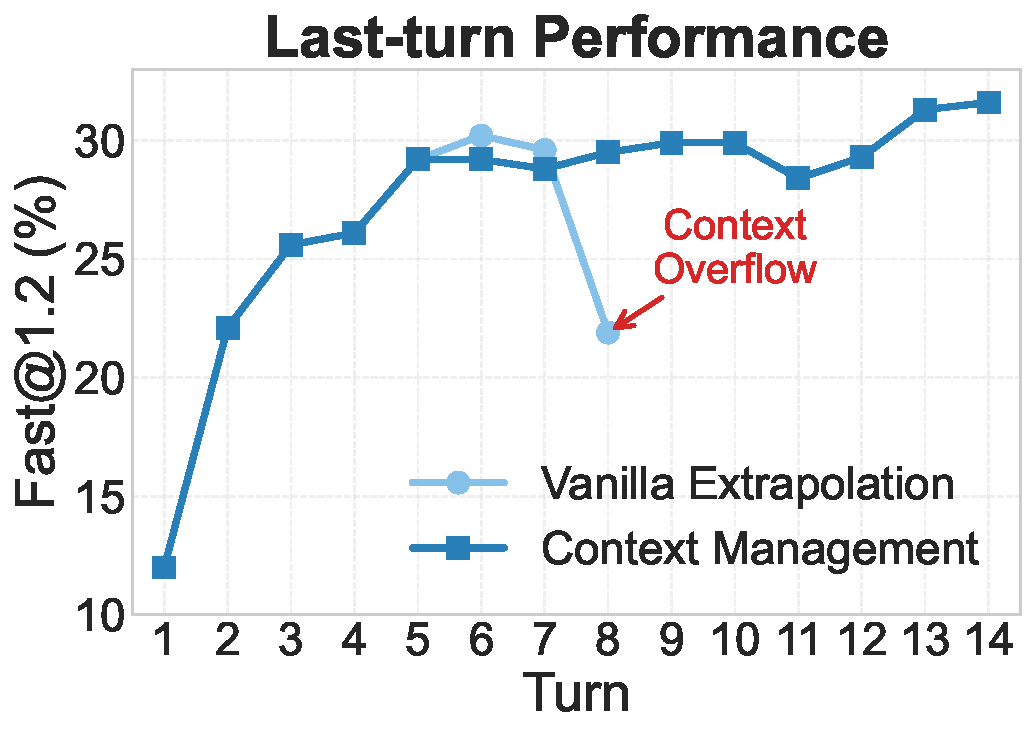
\includegraphics[width=\linewidth]{figures/tts/last_turn.pdf}
%     % \vspace{-2mm} % 可选：压缩上下空隙
%   \end{minipage}\hfill
%   \begin{minipage}[t]{0.49\columnwidth}
%     \centering
%     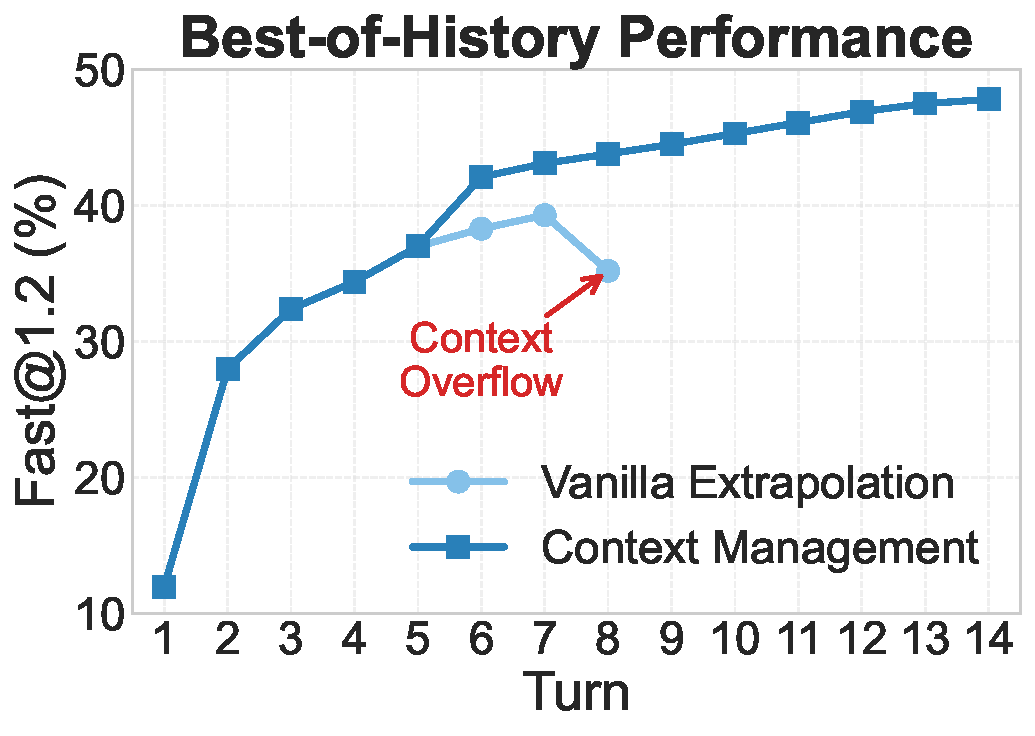
\includegraphics[width=\linewidth]{figures/tts/best_of_history.pdf}
%   \end{minipage}

%   \caption{Test-time scaling experiments using \kernel-14B on Last-turn performance and best-of-history performance. Vanilla Multi-turn scales the turn number directly. Context management variant keeps all history turns but only appends 4 turns with the best rewards as context.}
%   \label{fig:tts}
% \end{figure}

% We further use \kernel-14B with max length $32768$ to scale the turn number during inference via two approaches: vanilla extrapolation and with context management. We evaluate on the Fast@1.2 of last-turn and best-of-history. For vanilla multi-turn, we extrapolate the max turns from 3 in training to 8. The results in Figure~\ref{fig:tts} show that \kernel-14B can further improve Fast@1.2 with increasing max turns. Since simply extrapolating might hit the context window limit, we also conduct test-time scaling with context management, where we store all generated histories and keep a fixed turn history context window $w$ by selecting the best-of-$w$ rewards in all history turns and appending these selected turns as history when generating the next turn. As shown in Figure~\ref{fig:tts}, scaling the turns using context management with $w=4$, the best-of-history performance persistenly outperform vanilla extrapolation. And last-turn-performance slightly lags behind vanilla extrapolation when the turn is not large enough, since the vanilla extrapolation can view all previous histories during generation. But as the turn scales, both last-of-turn performance and best-of-history performance consistently outperform the peak performance of vanilla extrapolation.

\subsection{Test-time Scaling for Kernel Generation}
\label{sec:tts}
\begin{figure}[t!]
  \centering
  \begin{minipage}[t]{0.49\columnwidth}
    \centering
    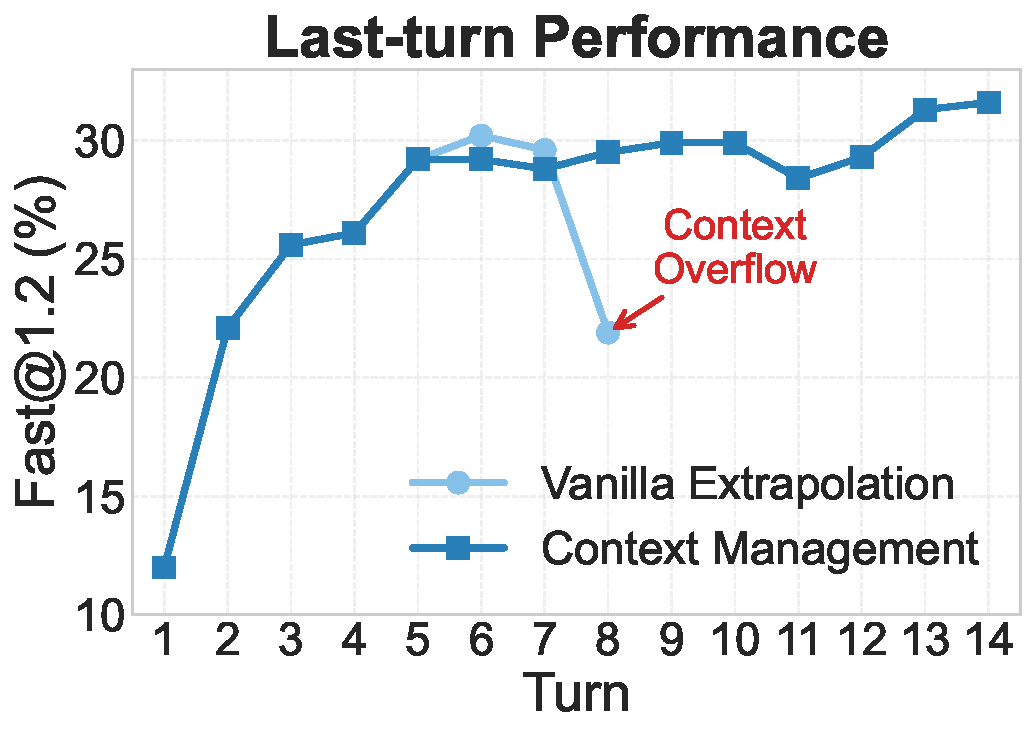
\includegraphics[width=\linewidth]{figures/tts/last_turn.pdf}
  \end{minipage}\hfill
  \begin{minipage}[t]{0.49\columnwidth}
    \centering
    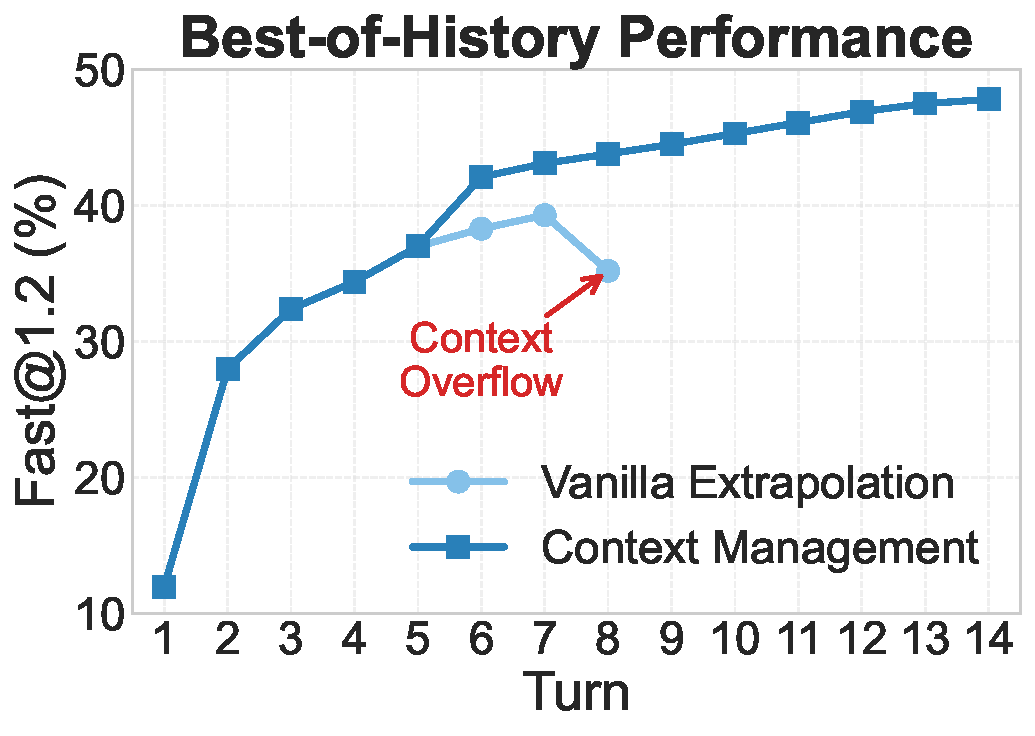
\includegraphics[width=\linewidth]{figures/tts/best_of_history.pdf}
  \end{minipage}
  % \vspace{-5pt}
  \caption{Test-time scaling with \kernel-14B. We report Fast@1.2 for the \textbf{last turn} (left) and \textbf{best-of-history} (right). Vanilla extrapolation increases the number of turns by appending all previous turns to the prompt. Context management stores the full history externally, but only includes the top-$w$ turns (by reward, $w{=}4$) in the prompt to fit context length.}
  % \vspace{-30pt}
  \label{fig:tts}
\end{figure}

We study sequential test-time scaling (STTS) by increasing the number of multi-turn refinement steps at inference time. We use \kernel-14B with a maximum context length of 32{,}768 tokens and evaluate two strategies: \textbf{vanilla extrapolation} and \textbf{context management}. We report two metrics: (i) Last-turn Fast@1.2, i.e., the Fast@1.2 achieved by the final generated kernel at turn $T$; and (ii) Best-of-history Fast@1.2, i.e., the best Fast@1.2 obtained among turns $\{1,\dots,T\}$. With STTS, our model even outperforms GPT-5/Claude-4.5-Sonnet in Kernelbench level-2 subset.

\textbf{Vanilla extrapolation} We directly extrapolate the number of refinement turns beyond training (trained with up to 3 turns) by appending the entire interaction history to the prompt at each turn. Figure~\ref{fig:tts} shows that increasing turns initially improves both last-turn and best-of-history performance. However, as $T$ grows, prompt length scales linearly and may approach the context limit, which can degrade performance.

\textbf{Context management} To scale $T$ without unbounded prompt growth, we store all turns in an external memory and maintain a fixed in-context window. Concretely, at each turn we select the top-$w$ turns with the highest rewards from the accumulated history and only append these selected turns as the prompt history for generating the next turn (we use $w{=}4$). As shown in Figure~\ref{fig:tts}, context management yields consistently stronger best-of-history performance and continues to improve as turns scale. Last-turn performance can be slightly lower at small $T$, since vanilla extrapolation can condition on the full history, but as $T$ increases, context management becomes strictly more reliable and surpasses the best performance achievable by vanilla extrapolation.

\subsection{Results on \texttt{torch.compile}}
\texttt{torch.compile} is an advanced PyTorch feature that captures PyTorch programs into a compiled computation graph and optimizes execution via operator fusion, code generation, and scheduling, among other compiler passes. While most prior work evaluates model-generated kernels only under Torch eager execution, we further validate both our models and frontier models under \texttt{torch.compile}, providing a substantially stronger and more practical assessment of speedups.

As shown in Table~\ref{tab:compile_table}, \kernel{} remains effective under the more challenging \texttt{torch.compile} setting and stays competitive with frontier models across the three levels. Because \texttt{torch.compile} already applies compiler optimizations, the headroom for additional gains is smaller than in eager mode; consequently, the absolute Fast@p numbers are generally lower for all models, including both ours and frontier models. Importantly, Fast@1 under \texttt{torch.compile} is also a stricter target: trivial ``lazy'' changes that may yield marginal improvements in eager execution typically do not surpass the optimized compiled baseline. These results suggest that our training methods generalize beyond eager-mode artifacts, and further scaling of data and model capacity is a promising direction to obtain larger improvements even on top of \texttt{torch.compile}.
\begin{table*}[t!]
\centering
\footnotesize
\setlength{\tabcolsep}{3.0pt}
\renewcommand{\arraystretch}{1.08}
\caption{Fast performance across levels under different thresholds (evaluated under \texttt{torch.compile}). Since \texttt{torch.compile} provides a strong optimized baseline, Fast@1 remains meaningful (unlike eager mode, where trivial ``lazy'' optimizations can inflate Fast@1).}
% \vspace{-6pt}
\resizebox{0.9\textwidth}{!}{%
\begin{tabular}{@{}c  *{4}{c} | *{4}{c} | *{4}{c} @{}}
\toprule
\multirow{2}{*}{\textbf{Model}}
& \multicolumn{4}{c}{\textbf{LEVEL1}}
& \multicolumn{4}{c}{\textbf{LEVEL2}}
& \multicolumn{4}{c}{\textbf{LEVEL3}} \\
\cmidrule(lr){2-5}\cmidrule(lr){6-9}\cmidrule(lr){10-13}
& \textbf{Fast$_{1}$} & \textbf{Fast$_{1.2}$} & \textbf{Fast$_{1.5}$} & \textbf{Fast$_{2}$}
& \textbf{Fast$_{1}$} & \textbf{Fast$_{1.2}$} & \textbf{Fast$_{1.5}$} & \textbf{Fast$_{2}$}
& \textbf{Fast$_{1}$} & \textbf{Fast$_{1.2}$} & \textbf{Fast$_{1.5}$} & \textbf{Fast$_{2}$} \\
\midrule

GPT-5
& $18.6$ & $8.0$ & $6.5$ & $5.5$
& $22.1$ & $3.6$ & $1.5$ & $1.0$
& $14.0$ & $4.0$ & $3.0$ & $1.0$ \\

Claude-4.5-Sonnet
& $10.0$ & $2.2$ & $2.0$ & $1.8$
& $20.5$ & $3.0$ & $0.0$ & $0.0$
& $12.0$ & $3.5$ & $0.5$ & $0.0$ \\

\kernel-8B
& $16$ & $3.0$ & $1.5$ & $8.4$
& $20.6$ & $0.8$ & $0.0$ & $0.0$
& $7.2$ & $2.3$ & $0.0$ & $0.0$ \\

\kernel-14B
& $17.8$ & $5$ & $3.3$ & $2.5$
& $23.5$ & $1.9$ & $0.0$ & $0.0$
& $9.2$ & $3$ & $0.0$ & $0.0$ \\

\bottomrule
\end{tabular}%
}
% \vspace{-0.6cm}
\label{tab:compile_table}
\end{table*}